\subsubsection{Concept 2}

This concept is similar to concept 1, however it attempts to reduce weight and cost by estimating
a depth map from a single camera using optical flow and IMU measurements. This method would depend on 
the drone moving enough to measure optical flow, this motion could be artificially introduced to the 
position control algorithm, or could be naturally occurring corrections for wind or controller error.

Zingg et al. have successfully used optical flow for obstacle detection and avoidance, however their application
was primarily concerned with distances in the periphery of the cameras view. Due to only considering 
the drones speed in the cameras z-axis, their method lost accuracy in the center of the frame \cite{zingg_mav_2010}.
This application would require perch detection anywhere in the frame, and so will need to consider all velocity components
in estimating depth.

To estimate depth using all velocity coponents, the following method is used:

\begin{itemize}
    \item Between two images captured at $t_1$ and $t_2 = T_1 + \Delta t$, the drone has average velocity $\bar{v}$.
    \item A given point in the image appears to move from $\bar{r_1}$ to $\bar{r_2}$ between the two frames,
            due to the motion of the camera. The magnitude of both vectors is assumed to be similar, and 
            approximately equal to $D$, the distance to the object.
    \item The displacement of the drone between the two images is $\bar{d_1} = \bar{v} \Delta t$.
    \item The scene will appear to move the same distance in the opposite direction from the perspective 
            of an assumed stationary camera. This displacement is $\bar{d_2} = -\bar{d_1}$.
    \item Using Farneback optical flow, which provides dense estimates of pixel displacement $\bar{OF}$,
            a pixel coordinate $\bar{p_1}$ in the image at $$t_1$$ can be matched to another pixel $\bar{p_2}$
            at $t_2$ as $\bar{p_2} = \bar{p_1} + \bar{OF}$
    \item The angle between $\bar{p_1}$ and $\bar{p_2}$ is equal to the angle between $\bar{r_1}$ and $\bar{r_2}$,
            and can be found using the dot product of $\bar{p_1}$ and $\bar{p_2}$.
    \item Using the law of cosines and the assumption that $|\bar{r_1}| \approx |\bar{r_2}| \approx D$,
            $D$ can be estimated using equation \ref{eqn:dist_modified}
\end{itemize}

Note that in the process used by Zingg et al. \cite{zingg_mav_2010} a rotation is applied to the optical flow
vectors which removes optical flow caused by the rotation of the camera(as this optical flow is independent of
distance, and therefore provides no useful information). The same step is also applied to the optical flow vectors
used here, before estimating distance.

\begin{eqn}[H]
    \begin{equation}
        \begin{aligned}
            \label{eqn:dist_modified}
            cos(\theta) = \frac{\bar{p_1} \cdot \bar{p_2}}{|\bar{p_1}|  |\bar{p_2}|}
            \\
            D = \sqrt{\frac{(\Delta t |\bar{v}|)^2}{2(1 - cos(\theta))}}
        \end{aligned}
    \end{equation}
    Where:
    \begin{itemize}
        \item $\bar{v}$ is the average velocity over timestep $\Delta t$.
        \item $\bar{p_1}$ is a pixel coordinate in the first image.
        \item $\bar{p_2}$ is the pixel coordinate that optical flow identifies 
                as matched to the coordinate $\bar{p_1}$.
    \end{itemize}
\end{eqn}

\paragraph{Budget}

An IMU is included in the budget for this experimental project, however it would not need to be a part
of device if used on a real drone, as most drones already have an IMU built into their control system.

\begin{table}[ht]
    \centering
    \caption{Estimated budget for the optical flow sensing design.}
    \label{tab:flow}


    \begin{spreadtab}{{tabular}{|c|c|c|c||c|}}
        \hline
        @Item                       & @Supplier                                                                                                         & @Unit Cost (USD) & @Quantity & @Total Cost (USD) \\
        \hline
        @SMA Wire                   & @\href{https://www.kelloggsresearchlabs.com/product/round-wire/}{Kelloggs Research Labs}                          & 15.99 & 1 & [-1,0] * [-2,0] tag(start) \\
        @Mechanical Materials and Fabrication & @-                                                                                                      &     0 & 1 & [-1,0] * [-2,0] tag(pretax)\\
        @Tax                        & @- & sum(cell(start):cell(pretax)) * 0.07 & 1 & [-1,0] * [-2,0] tag(posttax) \\
        @Misc. Spares               & @- & sum(cell(start):cell(posttax)) * 0.2 & 1 & [-1,0] * [-2,0] tag(end) \\
        \hline
        \multicolumn{4}{|c||}{@Total} & sum(cell(start):cell(end)) \\
        \hline
    \end{spreadtab}
\end{table}

\paragraph{Evaluation}

There are two theoretical issues with this design. The first is that it assumes the scene in the camera to be stationary;
that the only source of optical flow is the motion of the drone. That assumption will not often hold when viewing a wind
blown branch or power line. The other issue is that the example use case in Zingg et al. \cite{zingg_mav_2010} is not 
computing a full depth image; it simply is estimating if objects are approaching closer on the left or right hand side
of the frame and generates a control signal to steer the opposite direction. The accuracy of this depth estimation is 
sufficient for steering down a straight hallway, but that does not mean it will produce a depth map sufficient to detect 
a straight line.

The modified depth estimation has been tested with one sample video from the Mid-Air dataset \cite{fonder_mid-air_2019}.
The velocity and pose ground truth data have been interpolated to the same sample rate as the video and depth frames.
Fig. \ref{fig:c2:depth} shows a sample frame from the ground truth data, 
and Fig. \ref{fig:c2:depth_est} shows an example depth estimate from this process.
The depth estimation process produces very large estimates in some locations,
which cause the displayed image to appear as all 0 to these large singularities
overshadowing other data in the image scaling. To ensure the image can be displayed with 
useful data, values in the estimated image with a depth of over 500m are set to \texttt{nan}.
Pixels set to \texttt{nan} appear white in the displayed image.

\begin{figure}[H]
    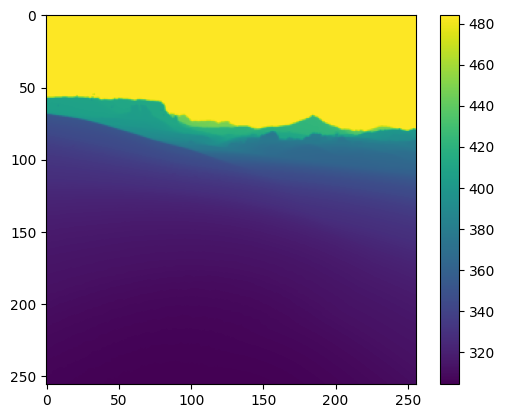
\includegraphics[width=\textwidth]{sections/sensor_concepts/ground_truth.png}
    \caption{Sample true depth image from the MidAir dataset. Depth values are in meters.
        Adapted from \cite{fonder_mid-air_2019}.}
    \label{fig:c2:depth}
\end{figure}

\begin{figure}[H]
    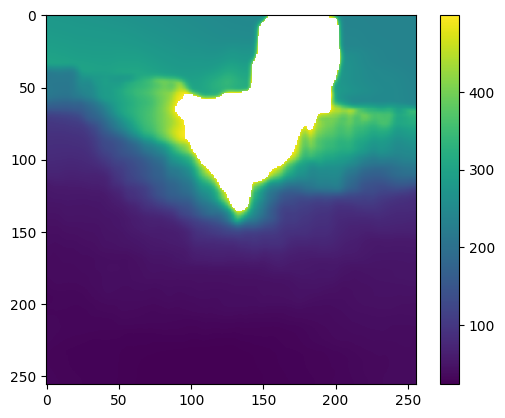
\includegraphics[width=\textwidth]{sections/sensor_concepts/estimate.png}
    \caption{Sample monocular depth estimation using the proposed method. Depth values are in meters.}
    \label{fig:c2:depth_est}
\end{figure}